\seclab{Results}{results}

In the following section, the results of the Lasso regression on the male and female data sets will be presented. In order to train the linear model, we need to develop a meaningful target vector for each of the images, based on the experimental input. This was done practically by taking the average of the inputted ages across all the experiments for each of the unique images. Also worth noting, is the fact that the degrees of freedom for the Lasso regression was capped at 40 and that a leave-one-out cross-validation was applied for both genders.

\subsection{Male Data Set}
We now present the results for the Lasso regression performed on the male data set. In \figref{M_Trace} we see a plot of the weights of the chosen eigenfaces (denoted by the different colours in the plot) as a function of decreasing regularization strength $\lambda$. As evident, the lower the strength, the greater the number of eigenfaces and the larger the weights become as discussed in \secref{methodandtheory}.

\begin{figure}[ht!]
    \centering
    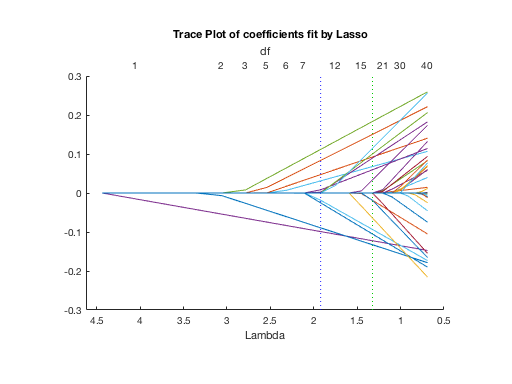
\includegraphics[width=0.85\linewidth]{fig/Trace_M_40.png}
    \caption{The weights of each eigenface plotted as a function of the $\lambda$ parameter for the male images.}
    \label{fig:M_Trace}
\end{figure}

In \figref{M_MSE} we see the evolution of the Mean Square Error (MSE) as a function of decreasing regularization strength $\lambda$. As evident, a local minimum has been found (local in the sense that we have constrained the Lasso to only consider up to 40 degrees of freedom) at $\lambda = 1.32$ corresponding to a MSE $= 189.4$ for the optimal model which was validated with leave-one-out cross-validation for the best possible estimate of the generalization error. 

\begin{figure}[ht!]
    \centering
    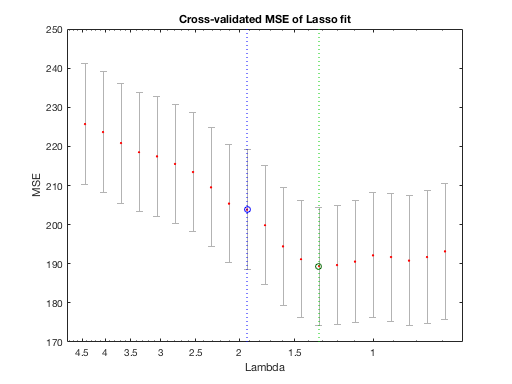
\includegraphics[width=0.8\linewidth]{fig/MSE_M_40.png}
    \caption{The Mean Squared Error (MSE) plotted as a function of the $\lambda$ parameter for the male images.}
    \label{fig:M_MSE}
\end{figure}

For the males a total of 16 eigenfaces were chosen with the optimal Lasso as evident in the left pane of \figref{M_Age}. Out of these 16 eigenfaces, 7 had negative weights associated with them whilst 9 had positive weights associated with them. The sign of the weights determine whether a positive projection onto one of the eigenfaces will correspond to an increase in the model's prediction of an age or not. The eigenfaces with negative weights can thus be thought of as young and vice versa.

\begin{figure}[ht!]
    \centering
    \begin{minipage}{0.49\textwidth}
    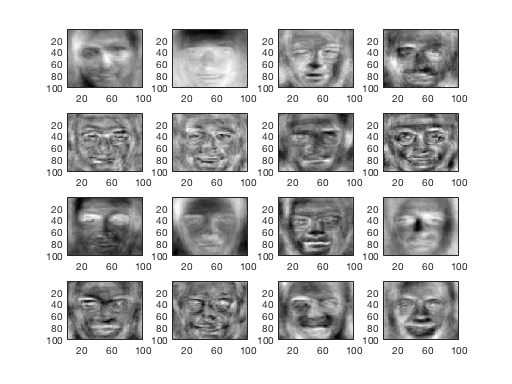
\includegraphics[width=1\linewidth]{fig/M_Lasso_40.png}
    \end{minipage}
    \begin{minipage}{0.49\textwidth}
    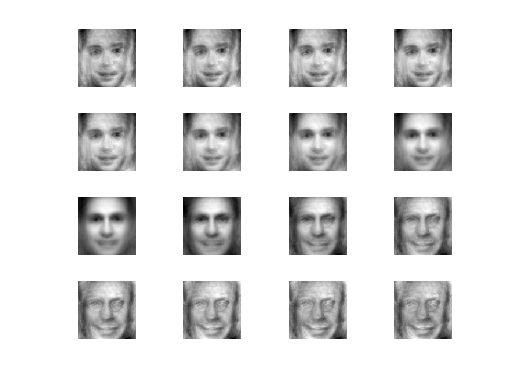
\includegraphics[width=1\linewidth]{fig/M_Age_40.png}
    \end{minipage}
    \caption{Left: The chosen eigenfaces from the Lasso regression ordered from the eigenface with the largest negative weight to the eigenface with the largest positive weight. Right: A linearly varying age based on the linear extension of the Lasso model for males, from the mean age minus 30 years to the mean age plus 30 years.}
    \label{fig:M_Age}
\end{figure}

Taking a closer look at the 16 chosen eigenfaces depicted in \figref{M_Age}, it becomes evident that the first couple of eigenfaces have "younger" characteristics in the sense that they have narrow noses, smoother skin and less noise surrounding the eyes. On the other hand, the last couple of eigenfaces seem to have wider noses and significantly more facial hair, which seems to indicate that facial hair makes you look older. It is also evident that the later eigenfaces have more glasses also indicating that the older a given man is the more likely he is to problems with sight.

Since we now have an understanding of how to interpret the chosen eigenfaces, we can proceed and try to look at the inverse problem, i.e., try to predict a face given an age. By \secref{methodandtheory}, we have assumed a linear relationship between the age and our eigenfaces, i.e., $y_i = \xxx_i^{\top} \www$. Since the feature vector $\xxx_i$ is just a straight line in a $M$-dimensional vector space and we know that only 16 eigenfaces contribute to the estimation of perceived age, we can write an observation $\xxx$ as a constant $\alpha$ times the contributing weights and their orthogonal complement (all of the non-contributing eigenfaces). Mathematically speaking we can write the linear relationship between targets and inputs as,
\begin{equation}\label{eq:alphaw}
    \begin{split}
        y_i &=\xxx_i^{\top} \www \\
            &=\qty(\alpha_i \www^{\top} + \www_{\perp}^{\top} )\www \\
            &= \alpha_i \www^{\top} \www \\
            &= \alpha_i \norm{\www}^2
    \end{split}
\end{equation}
where $\alpha_i= \dfrac{y_i}{\norm{w}^2}$ and hence we see that the age perceived is proportional to $\alpha$. By applying the thoughts behind \eqref{alphaw}, we can express a feature vector $\xxx_i= \alpha_i \www$ and thereby be able to reconstruct an image of arbitrary age. This has been done on the average male face (\figref{avgface}) for the average age (corresponding to the intercept of the Lasso regression) minus 30 years to the average age plus 30 years, the results of which can be seen in the right pane of \figref{M_Age}. Looking at the figure, similarities to the discoveries found from analysis of the plots in the left pane of \figref{M_Age} are evident. First and foremost, the eyes on the young male is clearly more well-defined. Likewise, another similarity is the appearance of glasses as the male is tweaked towards the elderly man in the bottom-right image. The third comment on the contributing eigenfaces holds for this evolution as well as the nose of the male clearly gets bigger as "time passes" (which is also a known fact for all human beings).

Another point to consider is the fact that the older/younger the image the less relative change there is in consecutive images which seems to indicate that the Lasso model has been constrained to such a degree that it gains better generalization error by guessing on ages close to the mean. In other words, we only see significant changes in the images for ages close to the mean age of approximately 43.7 years.

\subsection{Female Data Set}

We now present the results for the Lasso regression performed on the female data set. Similarly to the male Lasso, \figref{F_Trace} represents a plot of the weights of the chosen eigenfaces  as a function of decreasing regularization strength $\lambda$. Again, we see that the lower the strength, the greater the number of eigenfaces and the larger the weights become.

\begin{figure}[ht!]
    \centering
    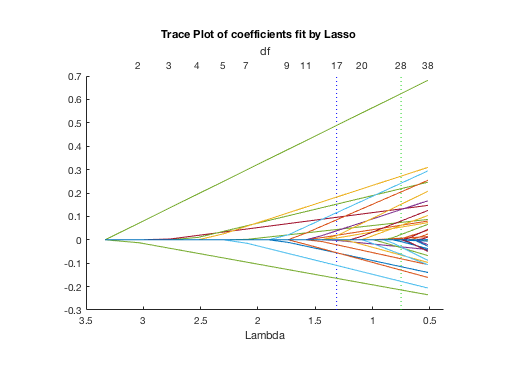
\includegraphics[width=0.85\linewidth]{fig/Trace_F_40.png}
    \caption{The weights of each eigenface plotted as a function of the $\lambda$ parameter for the female images.}
    \label{fig:F_Trace}
\end{figure}

In \figref{F_MSE} we see the evolution of the MSE as a function of decreasing regularization strength $\lambda$. As evident, a local minimum has been found at $\lambda = 0.75$ corresponding to MSE=169.3 for the optimal model. 

\begin{figure}[ht!]
    \centering
    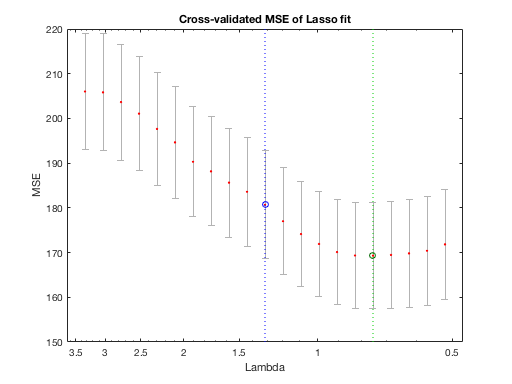
\includegraphics[width=0.8\linewidth]{fig/MSE_F_40.png}
    \caption{The Mean Squared Error (MSE) plotted as a function of the $\lambda$ parameter for the female images.}
    \label{fig:F_MSE}
\end{figure}

For the females a total of 28 eigenfaces were chosen, in which the first 12 have negative weights. In the left pane of \figref{F_Age}, the first 8 eigenfaces are the ones with the most negative weights and the final 8 eigenfaces are the ones with the highest positive weights. As for the males, we can see that the eigenfaces in the top left corner of the image patch seem to possess younger facial features such as small nose, smooth skin and large eyes. On the contrary we see that the eigenfaces in the lower right corner are more grainy which could correspond to wrinkles, also evident are the smaller eyes and larger noses. In the right pane of \figref{F_Age} we have displayed images of ages linearly varying from the Lasso intercept of 43.2 years minus 30 years to the intercept plus 30 years based on the average female face (\figref{avgface}). As for the males we see that the images in the extreme points of high/low age have similarities to the eigenfaces chosen by the Lasso regression. Also evident is the same trend with the variance being low and centered about the mean image, which as for the males, points towards a too harsh constraint on the part of the Lasso regression.

\begin{figure}[ht!]
    \centering
    \begin{minipage}{0.49\textwidth}
    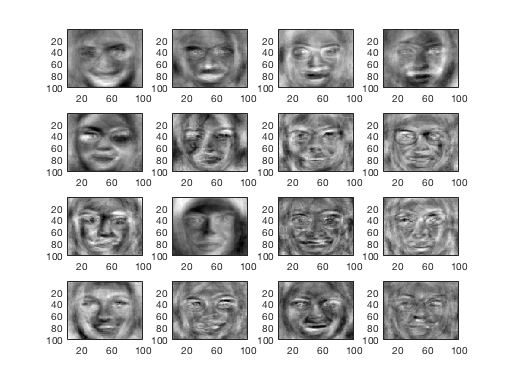
\includegraphics[width=1\linewidth]{fig/F_Lasso_40.png}
    \end{minipage}
    \begin{minipage}{0.49\textwidth}
    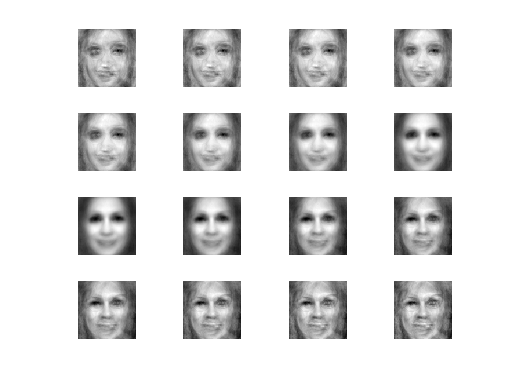
\includegraphics[width=1\linewidth]{fig/F_Age_40.png}
    \end{minipage}
    \caption{Left: The 16 most important chosen eigenfaces from the Lasso regression ordered from the eigenface with the largest negative weight to the eigenface with the largest positive weight. Right: A linearly varying age based on the linear extension of the Lasso model for males, from the mean age minus 30 years to the mean age plus 30 years.}
    \label{fig:F_Age}
\end{figure}